\documentclass[0-protokol.tex]{subfiles}
\begin{document}

\begin{table}[H] 
\centering
\setlength{\tabcolsep}{8pt}
\begin{tabular}{
    l
    S[table-format=2.1]
    S[table-format=1.1]
    S[table-format=1.4]
    S[table-format=1.4]
    S[table-format=1.2]
    S[table-format=1.2]
    S[table-format=1.2]
    S[table-format=1.2]
    S[table-format=2.1]
    S[table-format=2.1]
} \toprule
  & {$U$}            & {$\sigma_U$}     & {$I$}              & {$\sigma_U$}       & {$P$}            & {$\sigma_P$}     & {$\cos \varphi$} & {$\sigma_{\cos \varphi}$} & {$|\varphi|$}      & {$\sigma_{|\varphi|}$} \\
  & {$[\si{\volt}]$} & {$[\si{\volt}]$} & {$[\si{\ampere}]$} & {$[\si{\ampere}]$} & {$[\si{\watt}]$} & {$[\si{\watt}]$} & {$[]$}           & {$[]$}                    & {$[\si{\degree}]$} & {$[\si{\degree}]$}     \\ \midrule
R & 50.8             & 0.5              & 0.0504             & 0.0011             & 2.50             & 0.07             & 0.98             & 0.04                      & 12                 & 10                     \\
L & 51.0             & 0.5              & 0.0300             & 0.0005             & 0.50             & 0.07             & 0.33             & 0.05                      & 71.0               & 3.0                    \\
C & 49.6             & 0.5              & 0.1522             & 0.0026             & 0.12             & 0.07             & 0.017            & 0.010                     & 89.1               & 0.6                    \\ \bottomrule
\end{tabular}
\caption{Tabulka}
\label{tab:u1a}
\end{table}

\begin{table}[H] 
\centering
\setlength{\tabcolsep}{8pt}
\begin{tabular}{
    l
    S[table-format=2.1]
    S[table-format=1.1]
    S[table-format=1.4]
    S[table-format=1.4]
    S[table-format=1.2]
    S[table-format=1.2]
    S[table-format=1.2]
    S[table-format=1.2]
    S[table-format=2.1]
    S[table-format=2.1]
} \toprule
  & {$U$}            & {$\sigma_U$}     & {$I$}              & {$\sigma_U$}       & {$P$}            & {$\sigma_P$}     & {$\cos \varphi$} & {$\sigma_{\cos \varphi}$} & {$|\varphi|$}      & {$\sigma_{|\varphi|}$} \\
  & {$[\si{\volt}]$} & {$[\si{\volt}]$} & {$[\si{\ampere}]$} & {$[\si{\ampere}]$} & {$[\si{\watt}]$} & {$[\si{\watt}]$} & {$[]$}           & {$[]$}                    & {$[\si{\degree}]$} & {$[\si{\degree}]$}     \\ \midrule
R & 50.1             & 0.7              & 0.051              & 0.005              & 2.548            & 0.030            & 1.00             & 0.10                      & 0                  & 8                      \\
L & 50.3             & 0.7              & 0.030              & 0.005              & 0.594            & 0.015            & 0.39             & 0.07                      & 67                 & 4                      \\
C & 50.7             & 0.7              & 0.163              & 0.006              & 0.012            & 0.010            & 0.0015           & 0.0012                    & 89.92              & 0.07                   \\ \bottomrule
\end{tabular}


\caption{Tabulka}
\label{tab:u1d}
\end{table}

\begin{table}[H] 
\centering
\setlength{\tabcolsep}{8pt}
\begin{tabular}{
    S[table-format=1.0]
    S[table-format=2.1]
    S[table-format=1.1]
    S[table-format=1.3]
    S[table-format=1.3]
    S[table-format=1.3]
    S[table-format=1.3]
    S[table-format=1.2]
    S[table-format=1.2]
    S[table-format=2.0]
    S[table-format=2.0]
} \toprule
{$C$}                   & {$U$}            & {$\sigma_U$}     & {$I$}              & {$\sigma_U$}       & {$P$}            & {$\sigma_P$}     & {$\cos \varphi$} & {$\sigma_{\cos \varphi}$} & {$|\varphi|$}      & {$\sigma_{|\varphi|}$} \\
{$[\si{\micro\farad}]$} & {$[\si{\volt}]$} & {$[\si{\volt}]$} & {$[\si{\ampere}]$} & {$[\si{\ampere}]$} & {$[\si{\watt}]$} & {$[\si{\watt}]$} & {$[]$}           & {$[]$}                    & {$[\si{\degree}]$} & {$[\si{\degree}]$}     \\ \midrule
1                       & 51.1             & 0.7              & 0.015              & 0.005              & 0.243            & 0.012            & 0.32             & 0.11                      & 72                 & 7                      \\
2                       & 50.8             & 0.7              & 0.027              & 0.005              & 0.740            & 0.016            & 0.54             & 0.10                      & 57                 & 7                      \\
3                       & 50.3             & 0.7              & 0.035              & 0.005              & 1.213            & 0.020            & 0.69             & 0.10                      & 46                 & 8                      \\
4                       & 50.2             & 0.7              & 0.040              & 0.005              & 1.564            & 0.023            & 0.78             & 0.10                      & 39                 & 9                      \\
5                       & 50.1             & 0.7              & 0.043              & 0.005              & 1.800            & 0.024            & 0.84             & 0.10                      & 33                 & 11                     \\
6                       & 49.9             & 0.7              & 0.045              & 0.005              & 1.967            & 0.026            & 0.88             & 0.10                      & 29                 & 12                     \\
7                       & 49.9             & 0.7              & 0.046              & 0.005              & 2.083            & 0.027            & 0.91             & 0.10                      & 25                 & 14                     \\
8                       & 49.8             & 0.7              & 0.047              & 0.005              & 2.167            & 0.027            & 0.93             & 0.10                      & 22                 & 16                     \\
9                       & 49.8             & 0.7              & 0.047              & 0.005              & 2.233            & 0.028            & 0.95             & 0.11                      & 17                 & 20                     \\
10                      & 49.7             & 0.7              & 0.048              & 0.005              & 2.273            & 0.028            & 0.95             & 0.10                      & 18                 & 20                     \\ \bottomrule
\end{tabular}

\caption{Tabulka}
\label{tab:u4s}
\end{table}

\begin{table}[H] 
\centering
\setlength{\tabcolsep}{8pt}
\begin{tabular}{
    S[table-format=1.0]
    S[table-format=2.1]
    S[table-format=1.1]
    S[table-format=1.3]
    S[table-format=1.3]
    S[table-format=1.3]
    S[table-format=1.3]
    S[table-format=1.2]
    S[table-format=1.2]
    S[table-format=2.1]
    S[table-format=2.1]
} \toprule
{$C$}                   & {$U$}            & {$\sigma_U$}     & {$I$}              & {$\sigma_U$}       & {$P$}            & {$\sigma_P$}     & {$\cos \varphi$} & {$\sigma_{\cos \varphi}$} & {$|\varphi|$}      & {$\sigma_{|\varphi|}$} \\
{$[\si{\micro\farad}]$} & {$[\si{\volt}]$} & {$[\si{\volt}]$} & {$[\si{\ampere}]$} & {$[\si{\ampere}]$} & {$[\si{\watt}]$} & {$[\si{\watt}]$} & {$[]$}           & {$[]$}                    & {$[\si{\degree}]$} & {$[\si{\degree}]$}     \\ \midrule
1                       & 50.1             & 0.7              & 0.053              & 0.005              & 2.533            & 0.030            & 0.95             & 0.10                      & 17                 & 18                     \\
2                       & 50.1             & 0.7              & 0.060              & 0.005              & 2.555            & 0.030            & 0.85             & 0.08                      & 32                 & 8                      \\
3                       & 50.1             & 0.7              & 0.070              & 0.005              & 2.500            & 0.030            & 0.71             & 0.06                      & 45                 & 5                      \\
4                       & 50.4             & 0.7              & 0.083              & 0.005              & 2.577            & 0.031            & 0.62             & 0.04                      & 52.0               & 3.0                    \\
5                       & 50.5             & 0.7              & 0.096              & 0.005              & 2.583            & 0.031            & 0.533            & 0.031                     & 57.8               & 2.1                    \\
6                       & 50.5             & 0.7              & 0.110              & 0.005              & 2.581            & 0.031            & 0.465            & 0.024                     & 62.3               & 1.6                    \\
7                       & 50.7             & 0.7              & 0.110              & 0.005              & 2.591            & 0.031            & 0.465            & 0.024                     & 62.3               & 1.6                    \\
8                       & 50.6             & 0.7              & 0.140              & 0.006              & 2.591            & 0.031            & 0.366            & 0.016                     & 68.5               & 1.0                    \\
9                       & 50.6             & 0.7              & 0.155              & 0.006              & 2.589            & 0.031            & 0.330            & 0.013                     & 70.7               & 0.8                    \\
10                      & 50.8             & 0.7              & 0.171              & 0.006              & 2.595            & 0.031            & 0.299            & 0.011                     & 72.6               & 0.7                    \\ \bottomrule
\end{tabular}

\caption{Tabulka}
\label{tab:u4p}
\end{table}

\begin{table}[H] 
\centering
\setlength{\tabcolsep}{8pt}
\begin{tabular}{
    S[table-format=1.0]
    S[table-format=2.1]
    S[table-format=1.1]
    S[table-format=1.3]
    S[table-format=1.3]
    S[table-format=1.3]
    S[table-format=1.3]
    S[table-format=1.2]
    S[table-format=1.2]
    S[table-format=2.0]
    S[table-format=2.0]
} \toprule
{$C$}                   & {$U$}            & {$\sigma_U$}     & {$I$}              & {$\sigma_U$}       & {$P$}            & {$\sigma_P$}     & {$\cos \varphi$} & {$\sigma_{\cos \varphi}$} & {$|\varphi|$}      & {$\sigma_{|\varphi|}$} \\
{$[\si{\micro\farad}]$} & {$[\si{\volt}]$} & {$[\si{\volt}]$} & {$[\si{\ampere}]$} & {$[\si{\ampere}]$} & {$[\si{\watt}]$} & {$[\si{\watt}]$} & {$[]$}           & {$[]$}                    & {$[\si{\degree}]$} & {$[\si{\degree}]$}     \\ \midrule
1.0                     & 49.7             & 0.7              & 0.021              & 0.005              & 0.668            & 0.015            & 0.64             & 0.16                      & 50                 & 1                      \\
1.1                     & 49.7             & 0.7              & 0.023              & 0.005              & 0.826            & 0.017            & 0.72             & 0.16                      & 44                 & 1                      \\
1.2                     & 49.4             & 0.7              & 0.024              & 0.005              & 0.978            & 0.018            & 0.82             & 0.18                      & 34                 & 1                      \\
1.3                     & 49.3             & 0.7              & 0.026              & 0.005              & 1.107            & 0.019            & 0.86             & 0.17                      & 30                 & 1                      \\
1.4                     & 49.1             & 0.7              & 0.027              & 0.005              & 1.211            & 0.020            & 0.91             & 0.17                      & 24                 & 2                      \\
1.5                     & 49.0             & 0.7              & 0.028              & 0.005              & 1.291            & 0.020            & 0.94             & 0.17                      & 20                 & 2                      \\
1.6                     & 49.0             & 0.7              & 0.029              & 0.005              & 1.351            & 0.021            & 0.95             & 0.17                      & 18                 & 3                      \\
1.7                     & 48.9             & 0.7              & 0.029              & 0.005              & 1.391            & 0.021            & 0.98             & 0.17                      & 10                 & 5                      \\
1.8                     & 48.8             & 0.7              & 0.029              & 0.005              & 1.408            & 0.021            & 0.99             & 0.18                      & 5                  & 5                      \\
1.9                     & 48.7             & 0.7              & 0.029              & 0.005              & 1.421            & 0.021            & 1.00             & 0.18                      & 0                  & 5                      \\
2.0                     & 48.7             & 0.7              & 0.029              & 0.005              & 1.436            & 0.021            & 1.00             & 0.18                      & 0                  & 5                      \\
2.1                     & 48.8             & 0.7              & 0.029              & 0.005              & 1.423            & 0.021            & 1.00             & 0.18                      & 0                  & 5                      \\
2.2                     & 48.8             & 0.7              & 0.029              & 0.005              & 1.427            & 0.021            & 1.00             & 0.18                      & 0                  & 5                      \\
2.3                     & 48.7             & 0.7              & 0.029              & 0.005              & 1.417            & 0.021            & 1.00             & 0.18                      & 0                  & 5                      \\
2.4                     & 48.7             & 0.7              & 0.029              & 0.005              & 1.405            & 0.021            & 0.99             & 0.18                      & 6                  & 5                      \\
2.5                     & 48.8             & 0.7              & 0.029              & 0.005              & 1.391            & 0.021            & 0.98             & 0.17                      & 11                 & 5                      \\
2.6                     & 48.9             & 0.7              & 0.029              & 0.005              & 1.382            & 0.021            & 0.97             & 0.17                      & 13                 & 4                      \\
2.7                     & 48.7             & 0.7              & 0.029              & 0.005              & 1.368            & 0.021            & 0.97             & 0.17                      & 14                 & 4                      \\
2.8                     & 48.8             & 0.7              & 0.029              & 0.005              & 1.360            & 0.021            & 0.96             & 0.17                      & 16                 & 3                      \\
2.9                     & 48.9             & 0.7              & 0.028              & 0.005              & 1.346            & 0.021            & 0.98             & 0.18                      & 11                 & 5                      \\
3.0                     & 49.0             & 0.7              & 0.028              & 0.005              & 1.332            & 0.021            & 0.97             & 0.18                      & 14                 & 4                      \\
4                       & 48.9             & 0.7              & 0.027              & 0.005              & 1.224            & 0.020            & 0.93             & 0.18                      & 22                 & 2                      \\
5                       & 49.1             & 0.7              & 0.026              & 0.005              & 1.152            & 0.019            & 0.90             & 0.18                      & 26                 & 2                      \\
6                       & 49.0             & 0.7              & 0.026              & 0.005              & 1.103            & 0.019            & 0.87             & 0.17                      & 30                 & 2                      \\
7                       & 49.2             & 0.7              & 0.025              & 0.005              & 1.071            & 0.019            & 0.87             & 0.18                      & 29                 & 2                      \\
8                       & 49.2             & 0.7              & 0.025              & 0.005              & 1.047            & 0.018            & 0.85             & 0.17                      & 32                 & 1                      \\
9                       & 49.2             & 0.7              & 0.025              & 0.005              & 1.021            & 0.018            & 0.83             & 0.17                      & 34                 & 1                      \\
10                      & 49.2             & 0.7              & 0.025              & 0.005              & 1.007            & 0.018            & 0.82             & 0.17                      & 35                 & 1                      \\ \bottomrule
\end{tabular} 
\caption{Tabulka}
\label{tab:u5}
\end{table}

\begin{figure}[H]
\centering
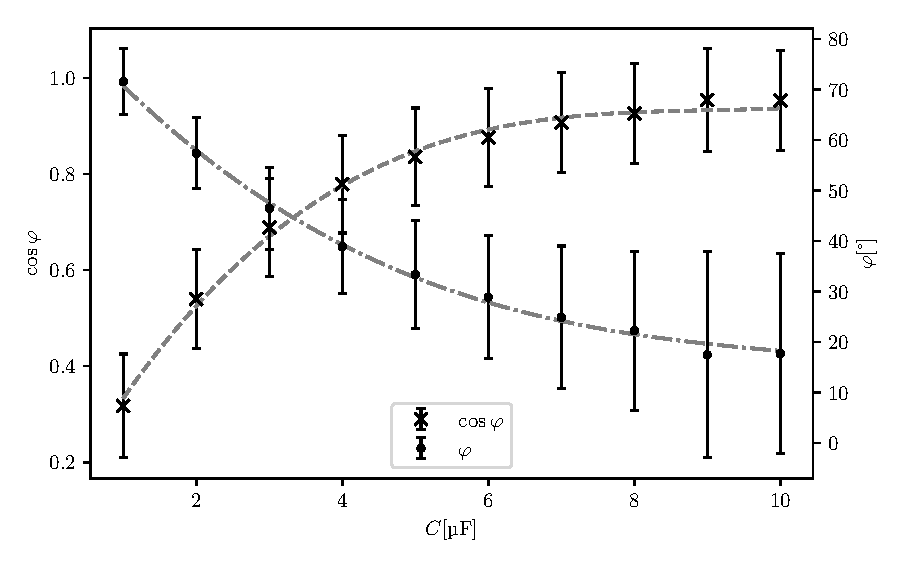
\includegraphics[]{u4s}
\caption{Závislost účiníku a fázového posunu sériového zapojení rezistoru a kondenzátoru}
\label{fig:u4s}
\end{figure}

\begin{figure}[H]
\centering
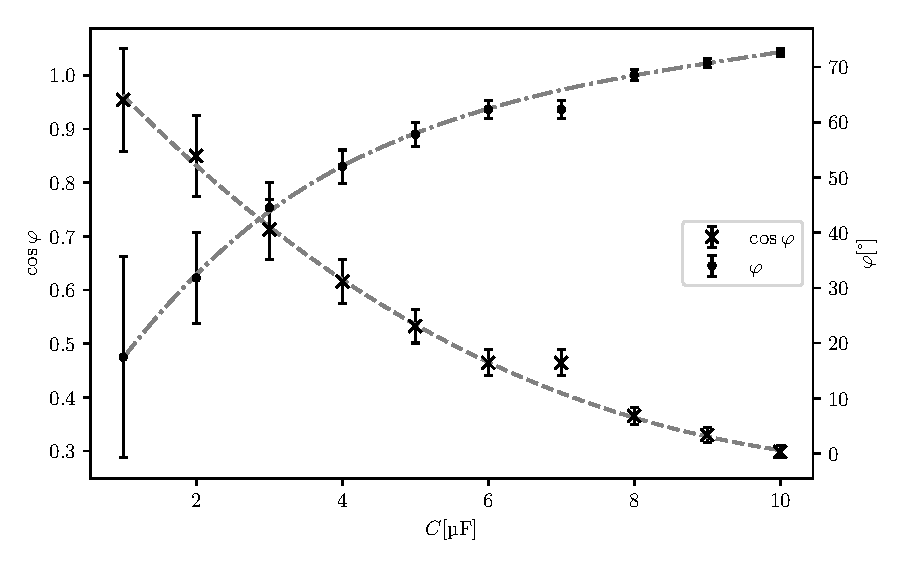
\includegraphics[]{u4p}
\caption{Závislost účiníku a fázového posunu paralelního zapojení rezistoru a kondenzátoru}
\label{fig:u4p}
\end{figure}

\begin{figure}[H]
\centering
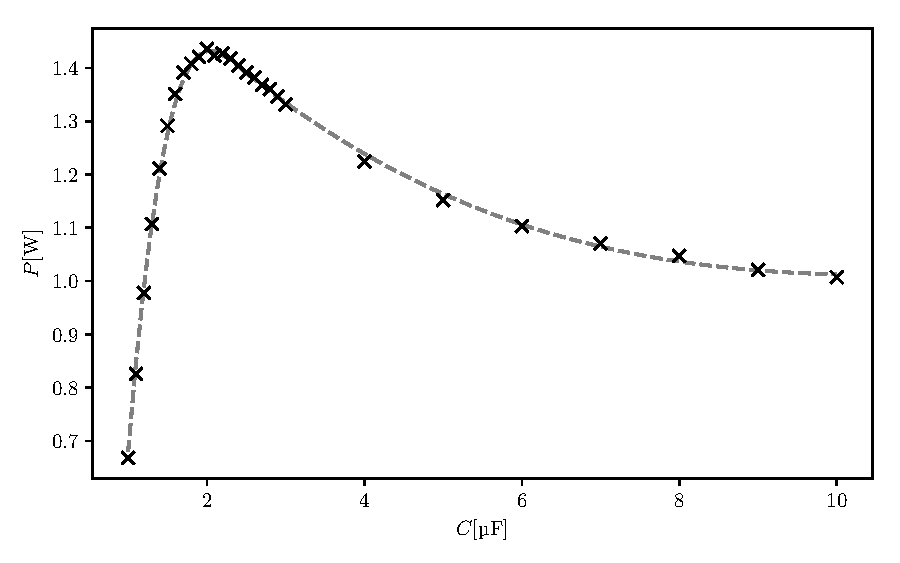
\includegraphics[]{u5p}
\caption{Průběh výkonu sériového RLC obvodu v závislosti na kapacitě}
\label{fig:u5p}
\end{figure}

\begin{figure}[H]
\centering
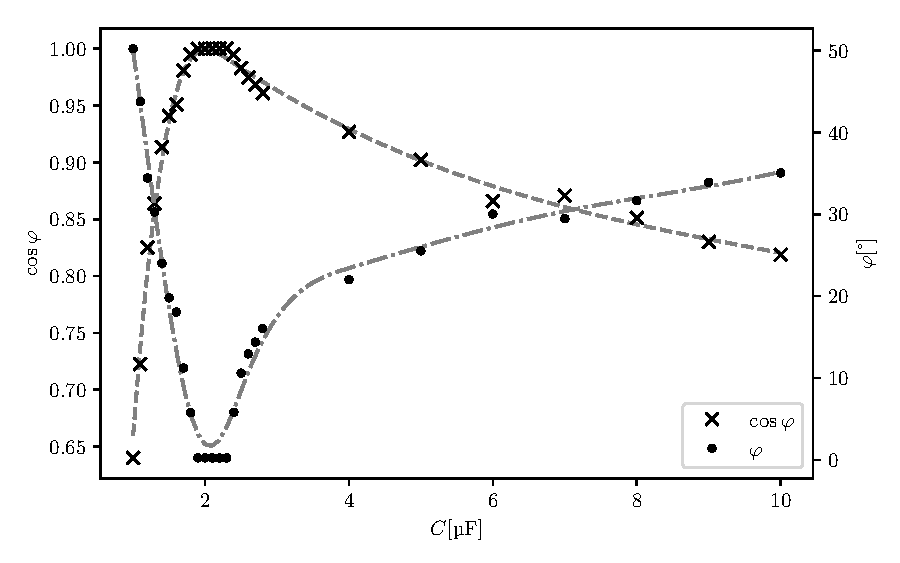
\includegraphics[]{u5uf}
\caption{Závislost účiníku a fázového posunu sériového RLC obvodu}
\label{fig:u5uf}
\end{figure}

\end{document}
